\documentclass[a4paper]{report}
% Shared preamble for the English probability and statistics documents.
% Based on the original course preamble. Compile with pdfLaTeX.
\usepackage[top=1.5cm,bottom=2cm,left=2cm,right=2cm]{geometry}
\usepackage[T1]{fontenc}
\usepackage{lmodern}
\usepackage[utf8]{inputenc}
\usepackage[english]{babel}

\usepackage{amsmath}
\usepackage{amssymb}
\usepackage{amsthm}
\usepackage{mathrsfs}
\usepackage{mathtools}
\usepackage{etoolbox}
\usepackage{tikz}
\usetikzlibrary{shapes.multipart,arrows.meta}
\usepackage{xcolor}
\usepackage{enumerate}
\usepackage[shortlabels]{enumitem}
\usepackage{hyperref}
\usepackage{version}
\usepackage{bbold}
\usepackage{fontawesome5}
\usepackage{fancyhdr}
\lfoot{}
\usepackage{natbib}
\usepackage{graphicx}
\usepackage{pdfpages}
\usepackage{authblk}
    
\usepackage{blindtext}
\usepackage{multicol}
\usepackage{collcell}
\usepackage{wrapfig}
\usepackage{blkarray}
\usepackage{cancel}
\usepackage{appendix}
\usepackage{float}
\makeatletter
\input{tex/assets/slashbox.sty}
\makeatother
\hypersetup{unicode,colorlinks,citecolor=red,filecolor=black,
  linkcolor=red,urlcolor=cyan}
\setlength{\columnsep}{1cm}
\pagenumbering{gobble}

\def\numtext#1{%
  \ifcase#1\or one\or two\or three\or four\or five\or six\or seven\or eight\or nine\or ten\or
  eleven\or twelve\or thirteen\or fourteen\or fifteen\or sixteen\or seventeen\or eighteen\or nineteen\or twenty\or Lots\fi}

\newcommand{\Byte}[1]{%
  \def\nodecontents{}%
  \foreach[count=\l] \k in {#1} {\xappto{\nodecontents}{\noexpand\nodepart{\numtext{\l}}\k}}%
  \node[rectangle split,rectangle split parts=8,rectangle split horizontal,draw] at (2,2){\nodecontents};}

\newcommand{\D}{{\mathrm{d}}}
\newcommand{\cE}{{\mathcal{E}}}
\newcommand{\cG}{{\mathcal{G}}}
\newcommand{\cX}{{\mathcal{X}}}
\newcommand{\cY}{{\mathcal{Y}}}
\newcommand{\cB}{{\mathcal{B}}}
\newcommand{\cF}{{\mathcal{F}}}
\newcommand{\cO}{{\mathcal{O}}}
\newcommand{\cS}{{\mathcal{S}}}
\newcommand{\cT}{{\mathcal{T}}}
\newcommand{\given}{\, \big| \,}
\newcommand{\cL}{{\mathscr{L}}}
\newcommand{\cD}{{\mathcal{D}}}
\newcommand{\cA}{{\mathscr{A}}}
\newcommand{\cP}{{\mathscr{P}}}
\newcommand{\cR}{{\mathscr{R}}}
\newcommand{\A}{{\mathcal A}}
\newcommand{\one}{\mathbb{1}}
\newcommand{\mathbbm}[1]{\mathbb{#1}}

\providecommand{\C}{}
\renewcommand{\C}{\mathbb C}
\newcommand{\R}{\mathbb R}
\newcommand{\Q}{\mathbb Q}
\newcommand{\N}{\mathbb N}
\newcommand{\T}{\mathbb T}
\newcommand{\F}{\mathbb F}
\renewcommand{\P}{\mathbb P}
\newcommand{\Z}{\mathbb Z}
\newcommand{\E}{\mathbb {E}}
\newcommand{\Pbb}[1]{\P\left( #1\right)}
\newcommand{\Ebb}[1]{\E\left[ #1\right]}

\newcommand{\lb}{\left (}
\newcommand{\rb}{\right )}
\newcommand{\lbb}{\left [}
\newcommand{\rbb}{\right ]}
\newcommand{\labs}{\left |}
\newcommand{\rabs}{\right |}
\newcommand{\lbrb}[1]{\lb #1 \rb}
\newcommand{\lbbrbb}[1]{\lbb#1\rbb}
\newcommand{\labsrabs}[1]{\labs#1\rabs}
\newcommand{\lbbrb}[1]{\lbb#1\rb}
\newcommand{\lbrbb}[1]{\lb#1\rbb}
\newcommand{\langlerangle}[1]{\langle#1\rangle}
\newcommand{\lbcurly}{\{}
\newcommand{\rbcurly}{\}}
\newcommand{\curly}[1]{\lbcurly#1\rbcurly}
\newcommand{\abs}{\labsrabs}
\newcommand{\ind}[1]{1_{#1}}
\newcommand{\indep}{\perp \!\!\! \perp}
\renewcommand{\d}{\, \mathrm{d}}

\newtheorem{theorem}{Theorem}
\newtheorem{problemCnt}{Lemma}
\theoremstyle{definition}
\newtheorem{problem}[problemCnt]{Problem}
\newtheorem{problembook}[problemCnt]{\faBook \,  Problem}
\newtheorem{problempencil}[problemCnt]{\faPencil* \,  Problem}
\newtheorem{problemstar}[problemCnt]{\faStar\,  Problem}
\newtheorem{problemstarpencil}[problemCnt]{\faStar \, \faPencil* \,   Problem}
\newtheorem{probleminteresting}[problemCnt]{\faSmile[regular] \,   Problem}
\newtheorem{solution}{Solution}

\newcommand{\fwcell}[1]{\makebox[\arraystretch\normalbaselineskip]{$#1$}}
\newenvironment{enumeratei}{\begin{enumerate}[(i)]}{\end{enumerate}}
\newenvironment{enumeratea}{\begin{enumerate}[(a)]}{\end{enumerate}}
\newenvironment{enumeraten}{\begin{enumerate}[\upshape 1.]}{\end{enumerate}}

% Compatibility helpers needed by a few files in the combined archive.
\AtBeginDocument{\noindent{\footnotesize English translation prepared with ChatGPT (OpenAI, GPT-6), 26 October 2026, for translation of the Bulgarian text into English and LaTeX formatting.
The Bulgarian originals remain the reference; translation may contain errors.}\par\smallskip}
\newcommand{\MissingGraphic}[1]{%
  \begin{center}\fbox{\parbox{0.82\linewidth}{\centering Missing source image: \texttt{#1}}}\end{center}}



\setlength{\emergencystretch}{3em}
\allowdisplaybreaks
\begin{document}


\noindent Probability and Statistics, 16.12.2023 \hfill Test 1

\hrulefill

\begin{it}
The exact grading formula depends on the results. As an approximation, use 2 plus the points earned. Time allowed: 3 hours. Good luck.

$m,n,k$ denote nonnegative integers.



\end{it}

\begin{problem}
    \begin{enumerate}
        \item (0.25 points) An urn contains 4 yellow, 5 green and 2 blue pebbles. After drawing one, a person rolls fair dice: one die for yellow, two for green and three for blue. Given that the dice total is 3, what is the probability that the pebble was green?

        \item (0.25 points)
        A fair die is rolled five times. Find the probabilities of\\
        \(A=\{\text{the maximum value is at least 3}\}\) and\\ \(B=\{\text{the product of all values is divisible by 10}\}\).


    \item (0.25 points)
    A person tosses two biased coins, each with heads probability \(1/3\). If their faces agree, they draw two balls from an urn containing 4 black and 2 white balls, winning as many BGN as the number of white balls drawn. If the coin faces differ, they roll a die and pay BGN 3 if it is even. Find the distribution of the profit and prove that the game is unfair. How much should the player pay for the game to be fair?

    \end{enumerate}
\end{problem}



\begin{problem}
   \begin{enumerate}
        \item (0.25 points) Let $X\sim Ge(p)$, i.e.
        $\P(X=k)=pq^k$ for
       $k \geq 0$;
        Prove the
        memoryless property:
        for every $m,n\geq0$, $\P(X>m+n|X\geq n)=\P(X>m)$.

        \item (0.25 points) Prove the converse:
        if $Y$ is a random variable
        taking values in
       $\{0,1,2, \dots\}$
        and, for all $m,n\geq0$, $\P(Y>m+n|Y\geq n)=\P(Y>m)$,
        then $Y\sim Ge(p)$
        for some $p\geq0$.

        \item (0.25 points)
        Let $X_1,\dots,
        X_n$ be independent
        random variables and
        define
        $X_{\min}:=\min\{X_1,\dots,X_n\}$ and
        analogously
       $X_{\max}$.
        Which expressions
       \[
       \P(X_1 > m)^n,
       \,\,
       \P(X_1 \leq m)^n,
       \,\,
              \P(X_1 \leq m),
       \,\,
              1-
       m  \P(X_1 > m)^n,
       \,\,
              1 -
           \P(X_1 > m)^n,
       (1-m)(1- \P(X_1 > m)^n)
       \]
        give the probabilities
        respectively
       $\P(X_{\min} \leq m)$
        and
       $\P(X_{\max} \leq m)$?
        Prove your answer.
        \item (0.25 points)
        Five
        fair
        dice are rolled together. Any die
        showing six
        is removed, and
        the others are rolled again until
        none remain.
        Let $K$ be the total number of
        rounds. Find
       $\P(K\leq n)$
        and $\P(K=n)$.


   \end{enumerate}


\end{problem}

\begin{problem}
    Genetic algorithms are a well-known class of heuristic algorithms.
    They begin with an initial
    population of chromosomes encoding possible
    solutions to a problem; over time, it
    evolves into a better population,
    hence their name.

    Specifically, suppose
    we wish to initialize
    $n$ chromosomes (Boolean vectors) of length
    $m$. All genes (vector entries/bits) are independent
    $Ber(1/2)$ random variables.

    \begin{enumerate}
        \item (0.5 points)
        What is the probability
        that all vectors are distinct? What is the expected
        total number of ones in
        all vectors?
        What is the expected number of
        vectors with fewer than $m/4$ zeros?
        \item (0.5 points)
        What is the expected number
        of repetitions, i.e.
        equal pairs of vectors among
        the $m$ vectors?
        Answer the same question
        if the vector entries are
        independent $Ber(p)$ with $p\in(0,1)$. For which $p$ is the expected
        number of repetitions minimized?

        \item (0.5 points) \textit{*Bonus: What is the expected
        number of unique vectors}?

        \item (0.5 points) \textit{**Bonus: For fixed $m$, what is the order of the smallest $n$
        for which the probability that all
        chromosomes are distinct is below $50\%$?}
\end{enumerate}

\end{problem}


\begin{problem}
A television lottery uses a random generator that selects an integer uniformly from 1 to 5. The game is as follows\footnote{\href{https://shorturl.at/bjlqU}{https://shorturl.at/bjlqU}}:
\begin{itemize}
    \item A random number is selected (2 in the example);
    \item The player may stop and win the amount below
    the last number drawn, or guess whether the next
    number will be smaller or larger. \textbf{Consecutive
    numbers are guaranteed to differ};
    \item An incorrect guess wins nothing and ends the game. After a correct guess,
    the player may continue, up to the grand prize of BGN 1000.
\end{itemize}


\begin{center}
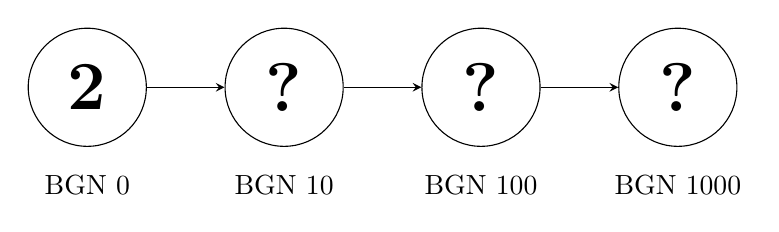
\begin{tikzpicture}[>=stealth, node distance=2.5cm, every loop/.style={}]
  \node[circle, draw, minimum size=1.5cm] (1) at (0,0) {\Huge \textbf{2}};
  \node[circle, draw, minimum size=1.5cm] (2) at (2.5,0) {\Huge \textbf{?}};
  \node[circle, draw, minimum size=1.5cm] (3) at (5,0) {\Huge \textbf{?}};
  \node[circle, draw, minimum size=1.5cm] (4) at (7.5,0) {\Huge \textbf{?}};


      \node[below] at (0,-1) {BGN 0};
      \node[below] at (2.5,-1) {BGN 10};
      \node[below] at (5,-1) {BGN 100};
      \node[below] at (3*2.5,-1) {BGN 1000};


  \draw[->] (1) -- (2) node[midway, above] {};
  \draw[->] (2) -- (3) node[midway, above] {};
  \draw[->] (3) -- (4) node[midway, above] {};

\end{tikzpicture}
\end{center}


\begin{enumerate}
    \item (0.5 points) Propose a strategy and calculate the winning probability and expected payoff if the player
    has decided to make exactly $k$ guesses, for $k=0,1,2,3$. Compare with independently choosing larger/smaller at random
    with probability $1/2$ each time.

    \item \textit{(0.25 points) Bonus: Give pseudocode solving the problem for numbers
    between $0$ and $n$, $m$ player choices, and prizes $c_0,\dots,c_n$.}

    \item \textit{(0.5 points) Bonus: Give pseudocode deciding whether
    stopping or guessing again is optimal after each round in the general game of part 2.}

\end{enumerate}




\end{problem}































































\end{document}
